\chapter{Framework} 
\label{Framework} % la etiqueta para referencias

%En los capitulos no usar mas de un nivel de subtitulos, i.e. subsection.
\section{Light as an Electromagnetic Wave} 
\label{Light is an EM Wave}

To understand how optical vortices work, and how they can be manipulated, first one must understand how light's behavior as an electromagnetic wave, or EM for short; it is important to emphasize that when talking about light, we are usually referring to a light beam. Light's propagation through space, as any other EM wave, can be modeled by equation (\ref{Light Equation}). For the purposes of this paper, phasor notation is preferred as it is useful to distinguish the light beam's real part ($A_0$ in the equation, and also referred to as \textit{intensity} or \textit{intensity field}) from its complex part ($\varphi_0$ in the equation, and also referred to as \textit{phase} or \textit{complex field}).

\begin{equation}
    U_0(r) = A_0e^{i\varphi}
    \label{Light Equation}
\end{equation}

This mathematical representation is mainly supported on Maxwell's four equations, or laws, \cite{Hecht_Optics-Appendix1}.

\begin{equation}
    \nabla \bigcdot \overrightarrow{\textbf{E}} = \frac{\rho}{\epsilon}
    \label{Gauss' Law for Electric Fields}
\end{equation}
\begin{equation}
    \nabla \bigcdot \overrightarrow{\textbf{B}} = 0
    \label{Gauss' Law for Magnetic Fields}
\end{equation}
\begin{equation}
    \nabla \times \overrightarrow{\textbf{E}} = -\frac{\partial \overrightarrow{\textbf{B}}}{\partial t}
    \label{Faraday's Law}
\end{equation}
\begin{equation}
    \nabla \times \overrightarrow{\textbf{B}} = \mu\sigma\overrightarrow{\textbf{E}}+\mu\epsilon\frac{\partial\overrightarrow{\textbf{E}}}{\partial t}
    \label{Ampere's Law}
\end{equation}

These laws unify the three great concepts of physics: electricity, magnetism and light; in particular, that light is an EM wave\footnotemark. In consequence, to comprehend how light propagates, we must understand what a wave is, and how it propagates. 

\footnotetext{Published by James Clerk Maxwell in 1865 in his work ``A Dynamical Theory of the electromagnetic Field'', where he added a term to Ampère's equation that had been published in 1861 ``On Physical Lines of Force'' which provided consistency with the other laws regarding dynamic fields, and added: ``The agreement of the results seem to show that light and magnetism are affections of the same substance, and that light is an electromagnetic disturbance propagated through the field according to electromagnetic laws''.}

In order to reach the model proposed in equation (\ref{Light Equation}), the concepts of \textit{wave} and \textit{field} and the \textit{wave equation} will be introduced, and alongside with them, the necessary conditions that must be met.

A wave is a spatial disturbance in a medium that carries energy and momentum. There are two\footnotemark{} main types of wave: mechanical and electromagnetic. Their difference lies in that mechanical waves require a physical medium for them to be propagated, while EM waves do not.

\footnotetext{There are other, much less common types of waves, like gravitational waves, plasma waves and quantum waves. The latter are very similar to mechanical waves, but instead follow the principles of quantum physics.}

A field, whether it is electric or magnetic, is a volume that depends on space and time, and can be ``constructed'' upon the variations of position that an arbitrary point within a wave experiences on each spatial axis $(x,y,z)$ as the wave travels. These displacements, which we will name $u(x,t)$, $u(y,t)$ and $u(z,t)$ respectively for each axis, are scalar functions that compose the field $\overrightarrow{\textbf{U}}(R,t)$, where $R = (x,y,z)$. The wave's dependencies on space and time exist because 1) it occupies a position in a volume or \textit{space} that 2) varies in time as it travels.

A simple illustration of this phenomenon can be seen in figure (\ref{fig:u_parameter_explanation}). Here, a mechanical wave is seen as it travels through a rope. The arbitrary point could be located anywhere within the rope, for example, at its center. The displacement this point will experience can be traced and then plotted. Naturally, the ``shape'' of the reference point's displacement should be wave-like, with respect to time. 

\begin{figure}[htbp]
    \centering
    \fbox{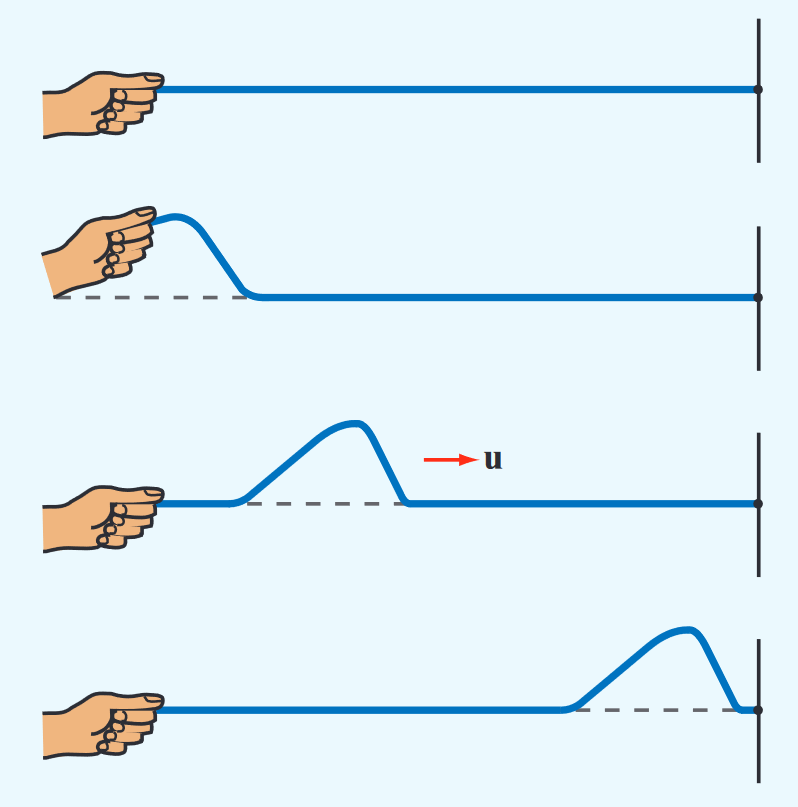
\includegraphics[width=8cm, height = 5.5cm]{images/c02/EM Waves/Wave_u_parameter.PNG}}
    \caption{Displacement $u$ of an arbitrary point as a wave travels through a rope in space and time \protect\cite{u_parameter_explanation-figure}.}
    \label{fig:u_parameter_explanation}
\end{figure}

\newpage
The wave equation describes this relationship better, and can be deduced from Ampère and Faraday's laws (refer to appendix \ref{WaveEquation_MaxwellEquations} for the mathematical demonstration). It describes the propagation of an EM wave through a medium, including vacuum.

\begin{equation}
    \nabla^2 \overrightarrow{\textbf{U}} = \frac{1}{c_0^2}\frac{\partial^2 \overrightarrow{\textbf{U}}}{\partial t^2}
    \label{Wave_Equation}
\end{equation}

Where $\overrightarrow{\textbf{U}}$ is the field\footnote{It could be either the electric field $\overrightarrow{\textbf{E}}$ or magnetic $\overrightarrow{\textbf{B}}$.}, $c_0$ is the propagation speed of the wave given by $c_0 = \frac{1}{\sqrt{\mu_0 \epsilon_0}}$, ($\mu_0$ and $\epsilon_0$ are the magnetic and electric permeability constants of the medium, respectively) and $t$ is time. Light in vacuum travels, naturally, at the speed of light, a number represented by the letter $c$ and equal to 299,792.458 $[\frac{km}{s}]$ (185,871,323.96 $[\frac{mi}{s}]$\footnote{NIST approximates a mile as $0.62 \times km$}) \cite{Hecht_Optics-Chapter3_EM_Waves} \cite{Speed_of_Light:NIST}.

Do note that the Laplacian is noted by the symbol $\nabla$ (read \textit{nabla}) and it represents the curl of the tridimensional field. It summarizes that the operation is being carried out in each spatial axis.

\begin{equation}
    \nabla^2 \overrightarrow{\textbf{U}} = \frac{\partial^2 \overrightarrow{\textbf{U}}}{\partial x^2} + \frac{\partial^2 \overrightarrow{\textbf{U}}}{\partial y^2} + \frac{\partial^2 \overrightarrow{\textbf{U}}}{\partial z^2}
    \label{Laplacian}
\end{equation}

\newpage
Then, by rewriting equation (\ref{Wave_Equation}) in terms of equation (\ref{Laplacian}), the following equation results.

\begin{equation}
    \frac{\partial^2 \overrightarrow{\textbf{U}}}{\partial x^2} + \frac{\partial^2 \overrightarrow{\textbf{U}}}{\partial y^2} + \frac{\partial^2 \overrightarrow{\textbf{U}}}{\partial z^2} = \frac{1}{c_0^2}\frac{\partial^2 \overrightarrow{\textbf{U}}}{\partial t^2}
    \label{Wave_Equation_Long}
\end{equation}

This equation shows that waves move in the same way of its shape, this means, in a sinusoidal motion. As it was stated before, if we were to plot the displacements of an arbitrary point in the field (left side of \ref{Wave_Equation_Long}), it would have the same shape as the wave itself (right side of \ref{Wave_Equation_Long}), corrected by the inverse of its speed to correctly match the magnitude as well. As for its direction, the symmetry described by Maxwell's equations denote that the disturbance will propagate in a direction that is symmetrical to both the electric $\overrightarrow{\textbf{E}}$ and magnetic $\overrightarrow{\textbf{B}}$ fields. Waves that propagate in this manner are called transverse waves, and is the case for all EM waves, light included. 

%What this equation is telling us is that the wave propagates with a profile resembling the one of the wave. In other words, the shape that it takes during the propagation (right side of \ref{Wave_Equation_Long}) is directly related with the wave's shape (left side of \ref{Wave_Equation_Long}), corrected by the inverse of its speed. As for its direction, the symmetry imposed by Maxwell's equations denote that the disturbance will propagate in a direction that is symmetrical to both the electric $\overrightarrow{\textbf{E}}$ and magnetic $\overrightarrow{\textbf{B}}$ fields. Waves that propagate in this manner are called transverse electromagnetic waves, or TEM for short.

\begin{figure}[htbp]
    \centering
    \fbox{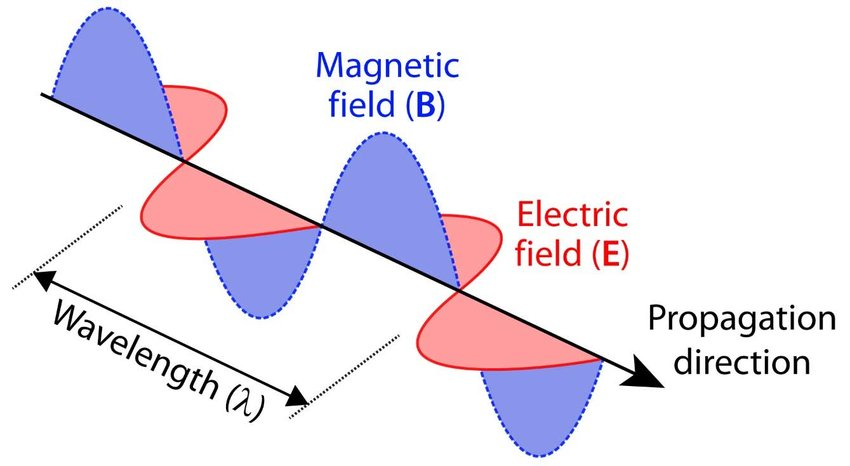
\includegraphics[scale=0.45]{images/c02/EM Waves/Light_EM_Wave.png}}
    \caption{Representation of a light wave propagating through space showing both of its fields, its wavelength ($\lambda$) and direction (black arrow) \protect\cite{Light_EM_Wave_Figure}. Its direction is given by the cross-product $\protect\overrightarrow{\textbf{E}} \times \protect\overrightarrow{\textbf{B}}$.}
    \label{fig:Light_EM_Wave}
\end{figure}

%Light is created from the thermonuclear reactions inside our Sun, as a consequence of the collision between hydrogen atoms, which in turn produce helium atoms. Moreover, light is one form of released energy from the an electron's shift between energy levels (either by yielding or receiving energy) within an atom; in other words, part of the energy differential is released in the form of photons\footnotetext{Other energy forms irradiated by the Sun are radiation, mainly ultraviolet and solar winds.}. These photons are known as the light particles, and they vibrate at different frequencies. 

Classical physics tell us that in all waves, frequency and wavelength are related by equation $\lambda = \frac{c_0}{f}$, where $f$ is the wave's frequency, $c_0$ it's speed and $\lambda$ it's wavelength. EM waves can have different wavelengths, or alternatively, frequencies, that can be seen in figure (\ref{fig:EM_Spectrum}). We humans perceive a portion of these wavelengths in the form of colors that compose the \textit{visible spectrum} of light. According to Hecht, ``light corresponds to the EM radiation in the narrow band from about $3.84 \times 10^{14}$ Hz to roughly $7.69 \times 10^{14}$ Hz'' \cite{Hecht_Optics-Visible_Light}. Some examples of colors and their respective wavelength and frequency, can be seen in table (\ref{tab:VisibleLight}).

\begin{figure}[htbp]
    \centering
    \fbox{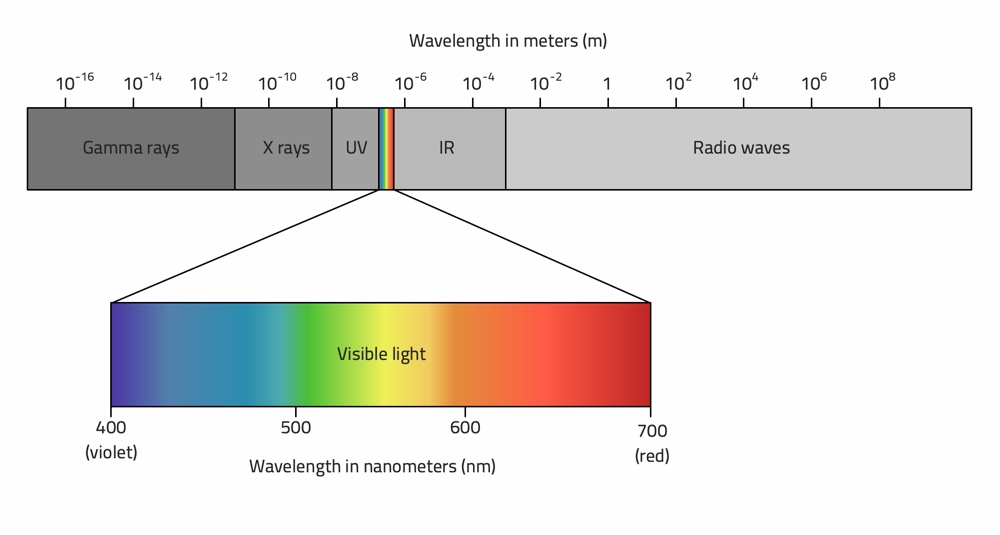
\includegraphics[width=11cm]{images/c02/EM Waves/EM_Spectrum.jpg}}
    \caption{EM Spectrum \protect\cite{EM_Spectrum-Figure}. The visible spectrum is encompassed between 390 and 780 [nm] although it is usually approximated to the range 400-700 [nm].}
    \label{fig:EM_Spectrum}
\end{figure}

\begin{table}[htbp]
    \centering
    \begin{tabular}{|l|c|c|}
    \hline
    \textbf{Color} & \textbf{$\lambda_0$ [nm]} & \textbf{$f$ [HZ]} \\ \hline
    Red           & 780-622                       & 384-482                  \\ \hline
    Orange        & 622-597                       & 482-503                  \\ \hline
    Yellow       & 597-577                       & 503-520                  \\ \hline
    Green          & 577-492                       & 520-610                  \\ \hline
    Blue           & 492-455                       & 610-659                  \\ \hline
    Violet        & 455-390                       & 659-769                  \\ \hline
    \end{tabular}
    \caption{Wavelength, in nanometers, and frequency, in terahertz, for some colors of the visible spectrum \protect\cite{Hecht_Optics-Visible_Light}. There is no international standard regarding the accuracy of these ranges are, as some variations of the upper and lower limits of the visible spectrum vary within the tens of nanometers.}
    \label{tab:VisibleLight}
\end{table}

\newpage
It is useful to distinguish what we perceive as light, as what might seem as a source of unique color, can actually be made out of multiple ones. For instance, sources like our Sun or a light bulb produce white light\footnote{The Sun looks yellow (instead of white) from Earth because of the scattering effect that our blue atmosphere has on ``rejecting'' blue and violet waves. However, this can be an extensive topic, worthy of its own.}, which is a combination of all colors, or wavelengths. On the other hand, monochromatic light are waves that share the same wavelength; for example, laser light is monochromatic. Therefore, in essence, although light can appear to be made out of multiple-frequency-waves, a single light wave is monochromatic.

\begin{figure}[htbp]
    \centering
    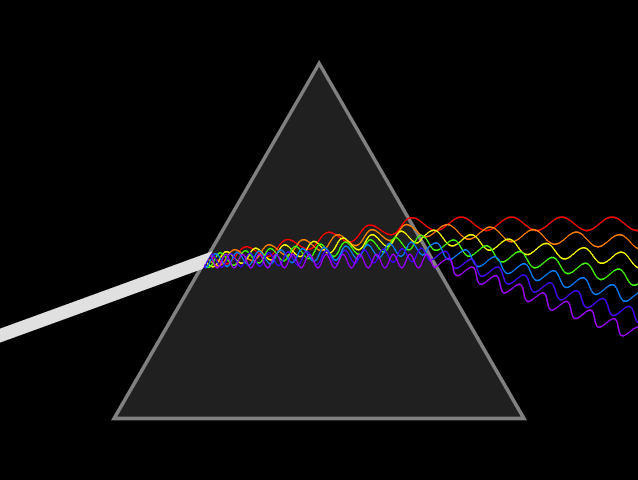
\includegraphics[width=6cm]{images/c02/EM Waves/Prism.PNG}
    \caption{Chromatic dispersion in a prism as a white light beam enters it. Sir Isaac Newton discovered in the late XVII century that a sunbeam impinging on a prism at a certain angle can disperse the colors composing in this beam and show them separately.}
    \label{fig:Prism}
\end{figure}

%Now that we have established some of light's properties and its behavior as an EM wave, we can continue with our demonstration.

Using this information to move on to our demonstration, we can notice that because light is a wave, a solution to its wave equation (\ref{Wave_Equation}) is another wave. Hence, the solutions we are looking for have the form of equation (\ref{Wave_Equation_Cartesian_Solution}).

%Como una única onda de luz es monocromática, las variaciones de campo que experimenta son sinusoidales, puesto que una solución a la ecuación de onda (\ref{Wave_Equation}) es la misma onda, multiplicada por el inverso de su velocidad al cuadrado, en este caso $c$ (o unos 90 kilómetros por segundos menos que $c$ dentro de la Tierra). En otras palabras, las soluciones son de la forma:

\begin{equation}
    U_0(r) = A_0\cos(\omega t + kr)
    \label{Wave_Equation_Cartesian_Solution}
\end{equation}

Where $A_0$ is the amplitude, given by $A_0 = A/r$, and $r = x^2 + y^2 + z^2$, $\phi = kr$ its phase and $k = \frac{2\pi}{\lambda} = \frac{\omega}{c_0}$. Finally, this equation can be rewritten as a phasor, which looks like our target equation (\ref{Light Equation}).

\begin{equation}
    U_0(r) = A_0e^{i\phi}
\end{equation}

\section{Optical vortices with Orbital Angular Momentum}
\label{c2:OAM}

In 1992 Allen et. al. published a paper showing that helically phased beams naturally carry an orbital angular momentum (OAM) that is $\ell$ times greater than the spin angular momentum's $\hbar$\footnote{Planck's constant, which is equal to $6.62607015\times 10^{-34}$ $[J\bigcdot s]$.} per photon \cite{Allen_OAM:1992}. Before this discovery, it was known that light can exert momenta upon the surfaces where it bounces off, pushing (linear momentum) or spinning them (spin angular momentum, or SAM). What is more, \textit{linear momentum} carries a momentum of $\hbar k_0$ per photon and, if the light beam is circularly polarized, a SAM of $\pm \hbar$ per photon. Simply put, this publication explained that light can also twist the receiving end \cite{Yao-Padgett:2011}.

Alison Yao and Miles Padgett exemplified these momenta in their work on OAM, to better understand them: ``[...] a laser pointer shone at a door can exert a torque about the hinge, albeit usually not enough to open it! However, when we discuss [OAM] [...] we seek to identify an angular momentum capable of twisting the door knob'' \cite{Yao-Padgett:2011-door_example}.

\begin{figure}[htbp]
    \centering
    \fbox{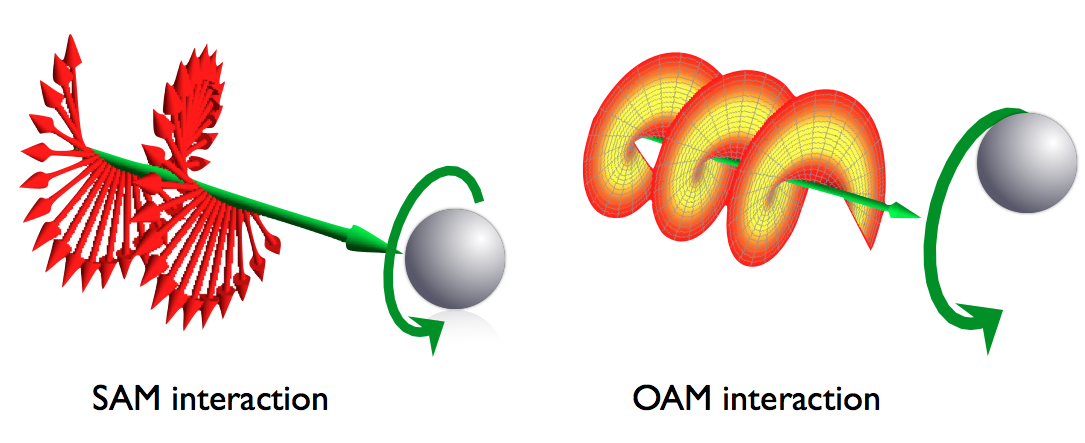
\includegraphics[width=10cm]{images/c02/OAM/SAM_OAM.png}}
    \caption{Comparison between SAM and OAM \protect\cite{Wikimedia:SAM_vs_OAM}}
    \label{fig:SAM_vs_OAM}
\end{figure}

One of the most remarkable features of beams that carry OAM (often referred to as OAM beams) is that they present a phase singularity running along its center that, in turn, is seen as a region of total darkness in intensity. As such, they resemble a vortex, which is defined as a region in a fluid that revolves around an axis line (e.g., water draining in a sink). If we think of light as the ``fluid'', then the beam would be an optical vortex, as its photons revolve around the optical axis. A projected OAM, or vortex, is shown in figure (\ref{fig:Example_OAM}).

%\begin{figure}[htbp]
%    \centering
%    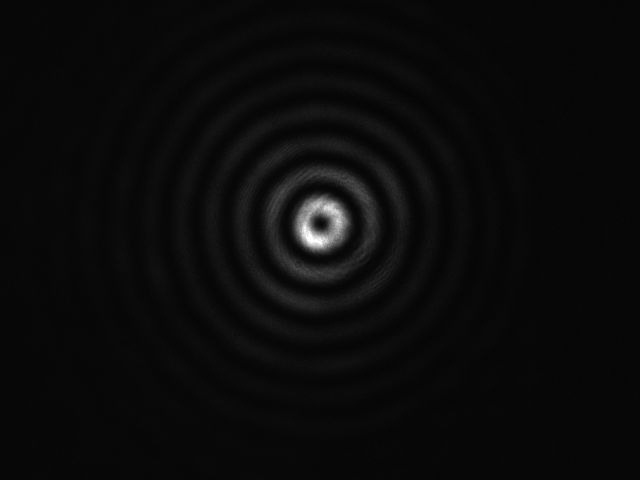
\includegraphics[width=7cm]{images/c02/OAM/OAM.png}
%    \caption{Real regular OAM beam projected onto a surface.}
%    \label{fig:Simple_OAM_Example}
%\end{figure}

\begin{figure}[htbp]
    \centering
    \begin{subfigure}[b]{0.45\textwidth}
        \centering
        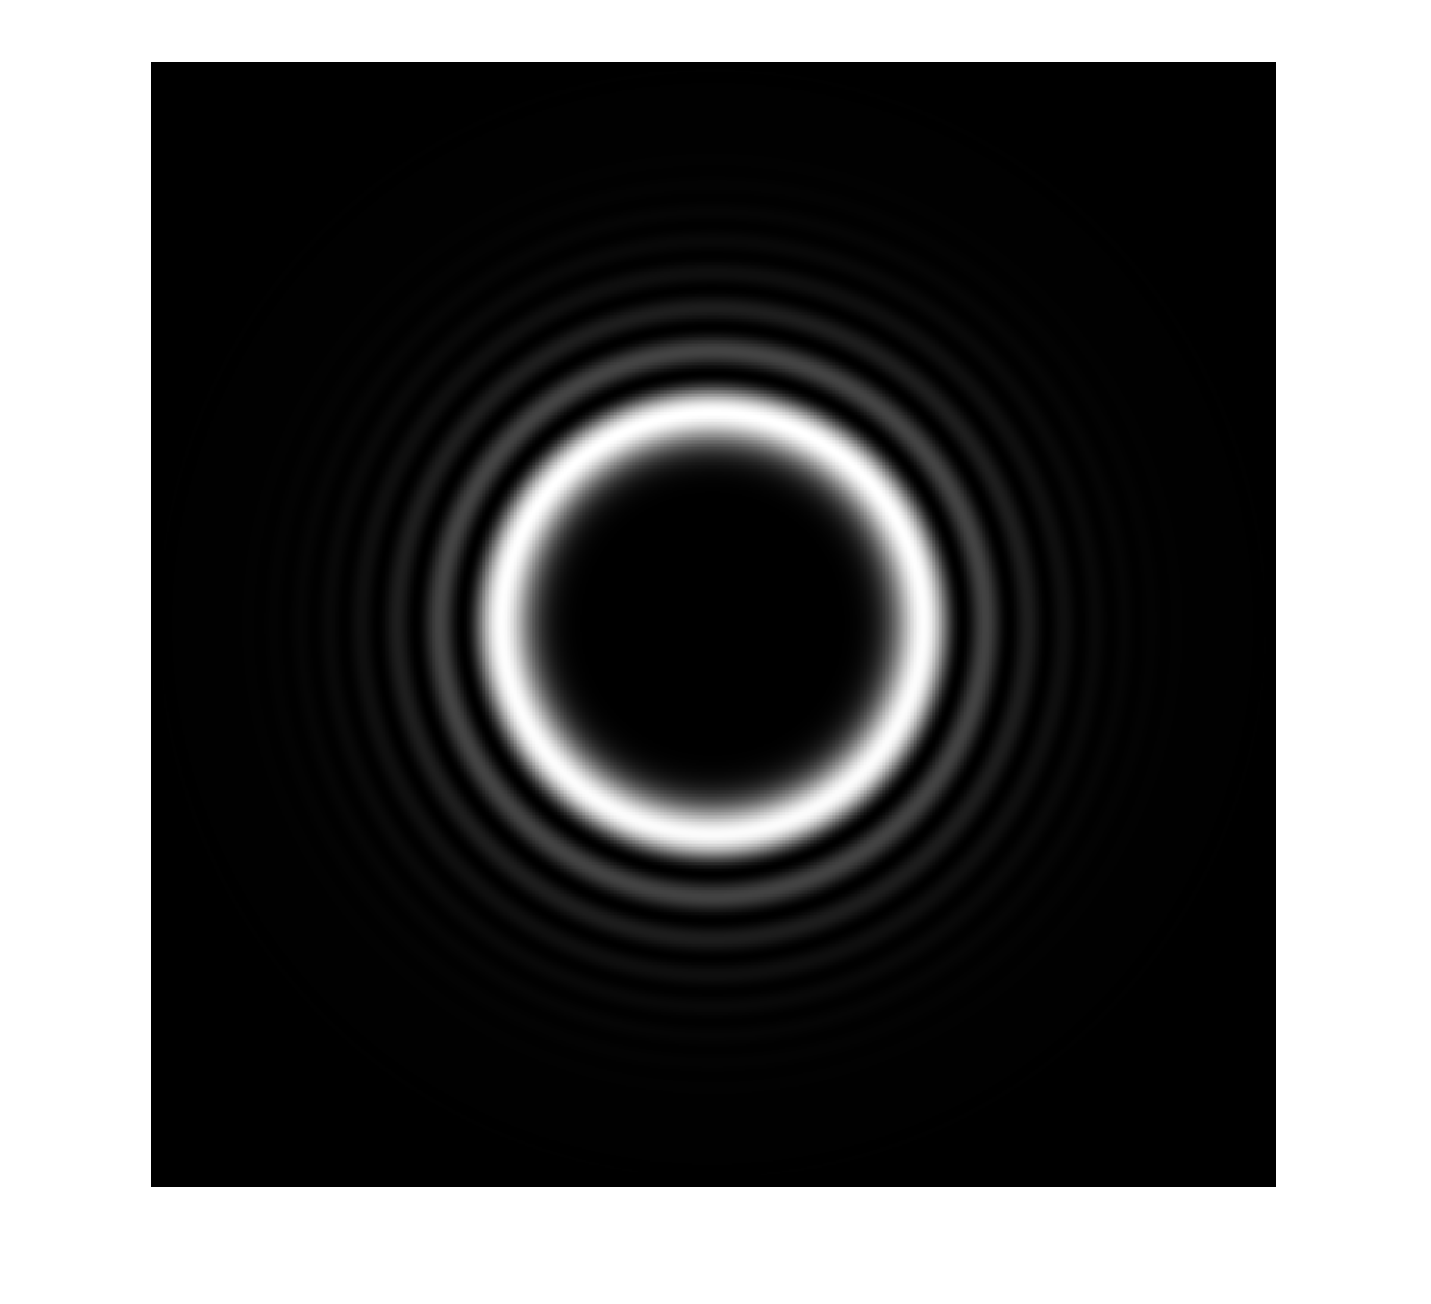
\includegraphics[width=\textwidth]{images/c02/OAM/Regular_OAM.eps}
        \caption{Regular vortex.}
    \end{subfigure}
    \hfill
    \begin{subfigure}[b]{0.45\textwidth}
        \centering
        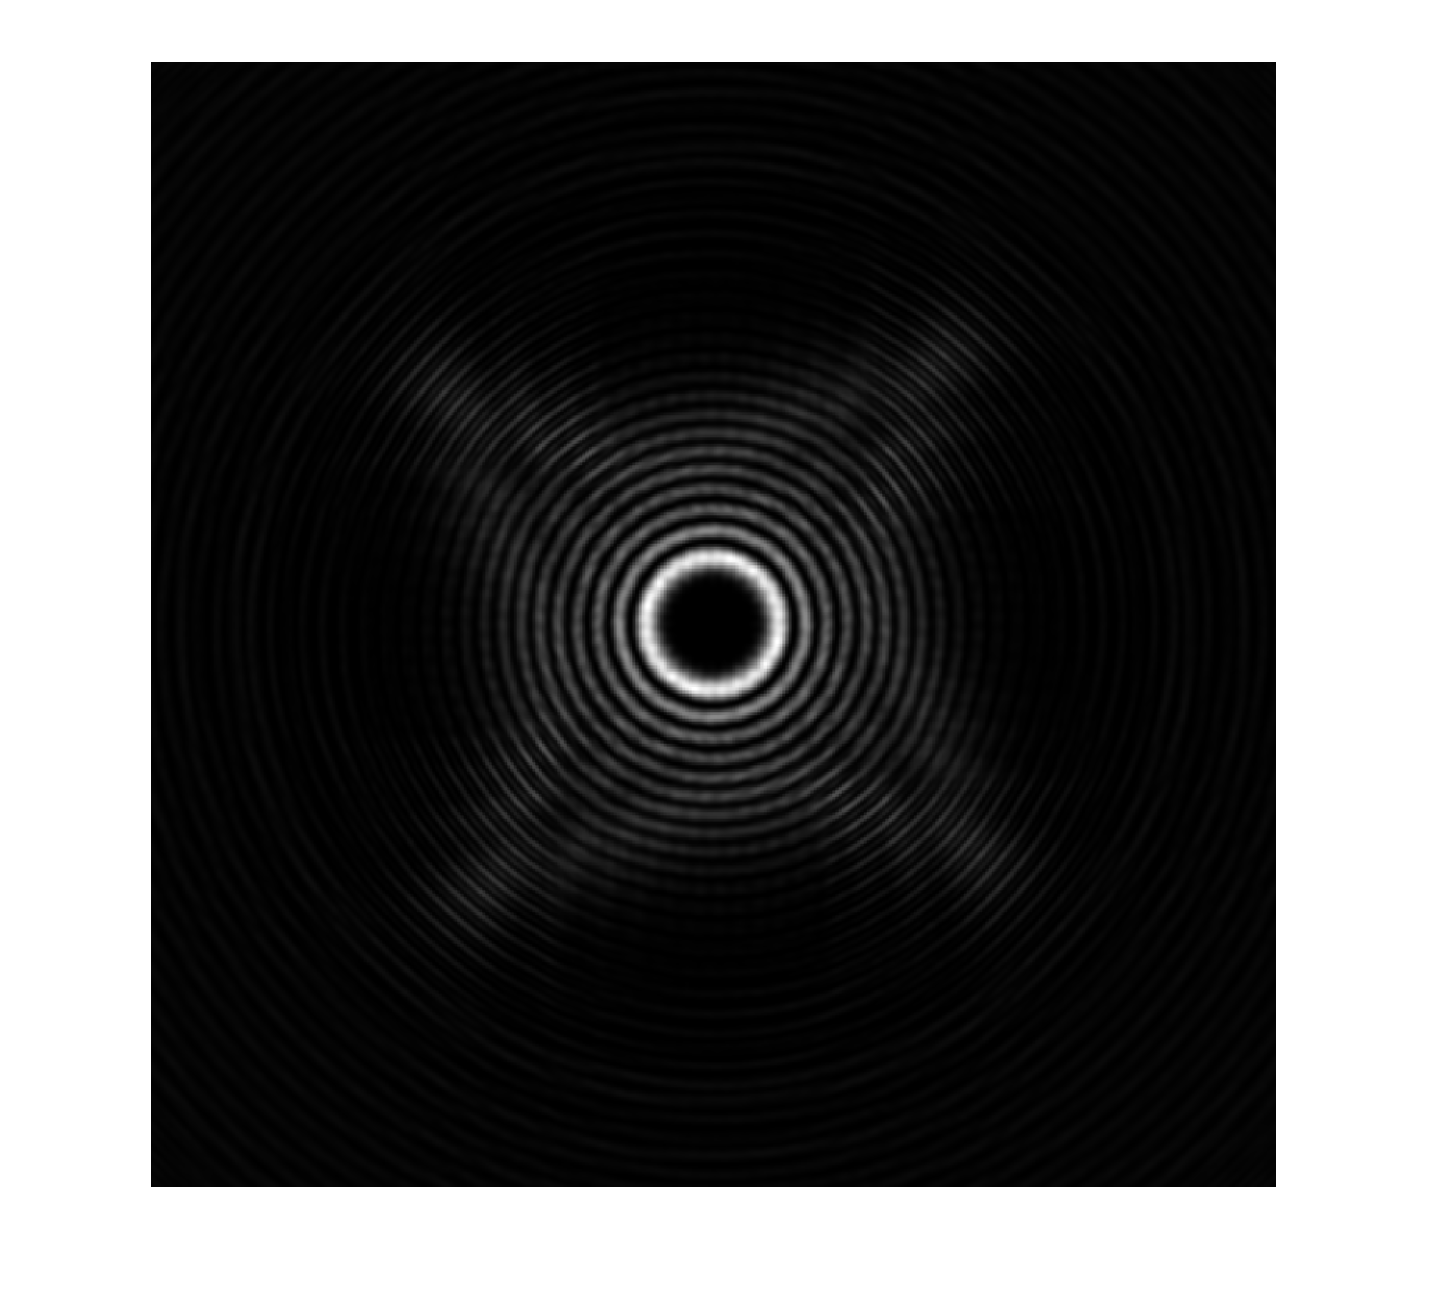
\includegraphics[width=\textwidth]{images/c02/OAM/OAM_10_40.eps}
        \caption{Perfect vortex.}
    \end{subfigure}
    \caption{Optical vortices produced from simulations (Own elaboration).}
    \label{fig:Example_OAM}
\end{figure}

The number $\ell$, the factor that amplifies the momentum of OAM with respect to the SAM, is designated \textit{topological charge} or \textit{state}. This number not only translates into the number of ``helices'' the corkscrew-like beam will have, but also correlates to its radial size and, as a consequence, to the size of the phase singularity. A representation of these beams in the midst of propagation can be seen in figure (\ref{fig:Different_OAM_Beams}).

%In contrast, \textit{perfect vortices} are a special type whose size, in theory, does not correlate to the state of the OAM; in other words, they are constant in size as they propagate \cite{Thesis_Herbert_PerfectVortices:2020}.

\begin{figure}[htbp]
    \centering
    \fbox{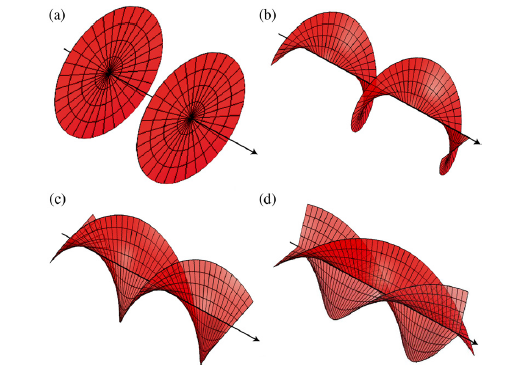
\includegraphics[width=9.5cm]{images/c02/OAM/OAM_topological_charge.PNG}}
    \caption{OAM beams of topological charges: (a) $\ell = 0$, (b) $\ell = 1$, (c) $\ell = 2$ and (d) $\ell = 3$. These illustrations show how OAM states differ from each other, disregarding their projections onto a surface \protect\cite{Yao-Padgett:2011}.}
    \label{fig:Different_OAM_Beams}
\end{figure}

There is another type of OAM: perfect vortices. They differ from regular ones in that their size does not correlate to the state of the OAM; furthermore, their size is constant throughout the propagation. Their intensity is defined by equation (\ref{eq:perfect_vortex_intensity}) \cite{Thesis_Herbert_PerfectVortices:2020}. 

\begin{equation}
    g_\ell (\rho,\theta) = \delta (\rho - \rho_0)e^{i\ell\theta}
    \label{eq:perfect_vortex_intensity}
\end{equation}

Where $\rho$ and $\theta$ are the polar coordinates of the beam's transversal section, $\delta$ is Dirac's delta function and $\rho_0$ the vortex's radius \cite{Kotlyar:16}.

On the other hand, regular OAM beams tend to grow in size and change in shape as they travel from the source towards infinity. At the very beginning, the beam does not resemble a beam like that of figure (\ref{fig:Example_OAM}), however as the distance $z$ increases, the more it resembles it. The beam will not only take this shape, but will also keep growing in radial size, which also means that its intensity fades away as the region the same light covers grows. As the beam approaches infinity, its shape will be even more static and its growth will also slow significantly.

A feature that both regular and perfect OAM beams share, is their intensity distribution. The lasers commonly used in optics have a Gaussian distribution, that is, very bright at its mean $\mu$ and fades at a rate related to its standard deviation $\sigma$. As figure (\ref{fig:Example_OAM}) shows, OAM beams can have rings. The intensity distribution, following that of a Gaussian, tends to concentrate most of the intensity in the smaller, most centered ring (also referred to as the main ring). The surrounding rings follow a Gaussian distribution, considering the ``skips'' they have between them. This is better illustrated in the following figure.

\begin{figure}[htbp]
    \centering
    \begin{subfigure}[b]{0.45\textwidth}
        \centering
        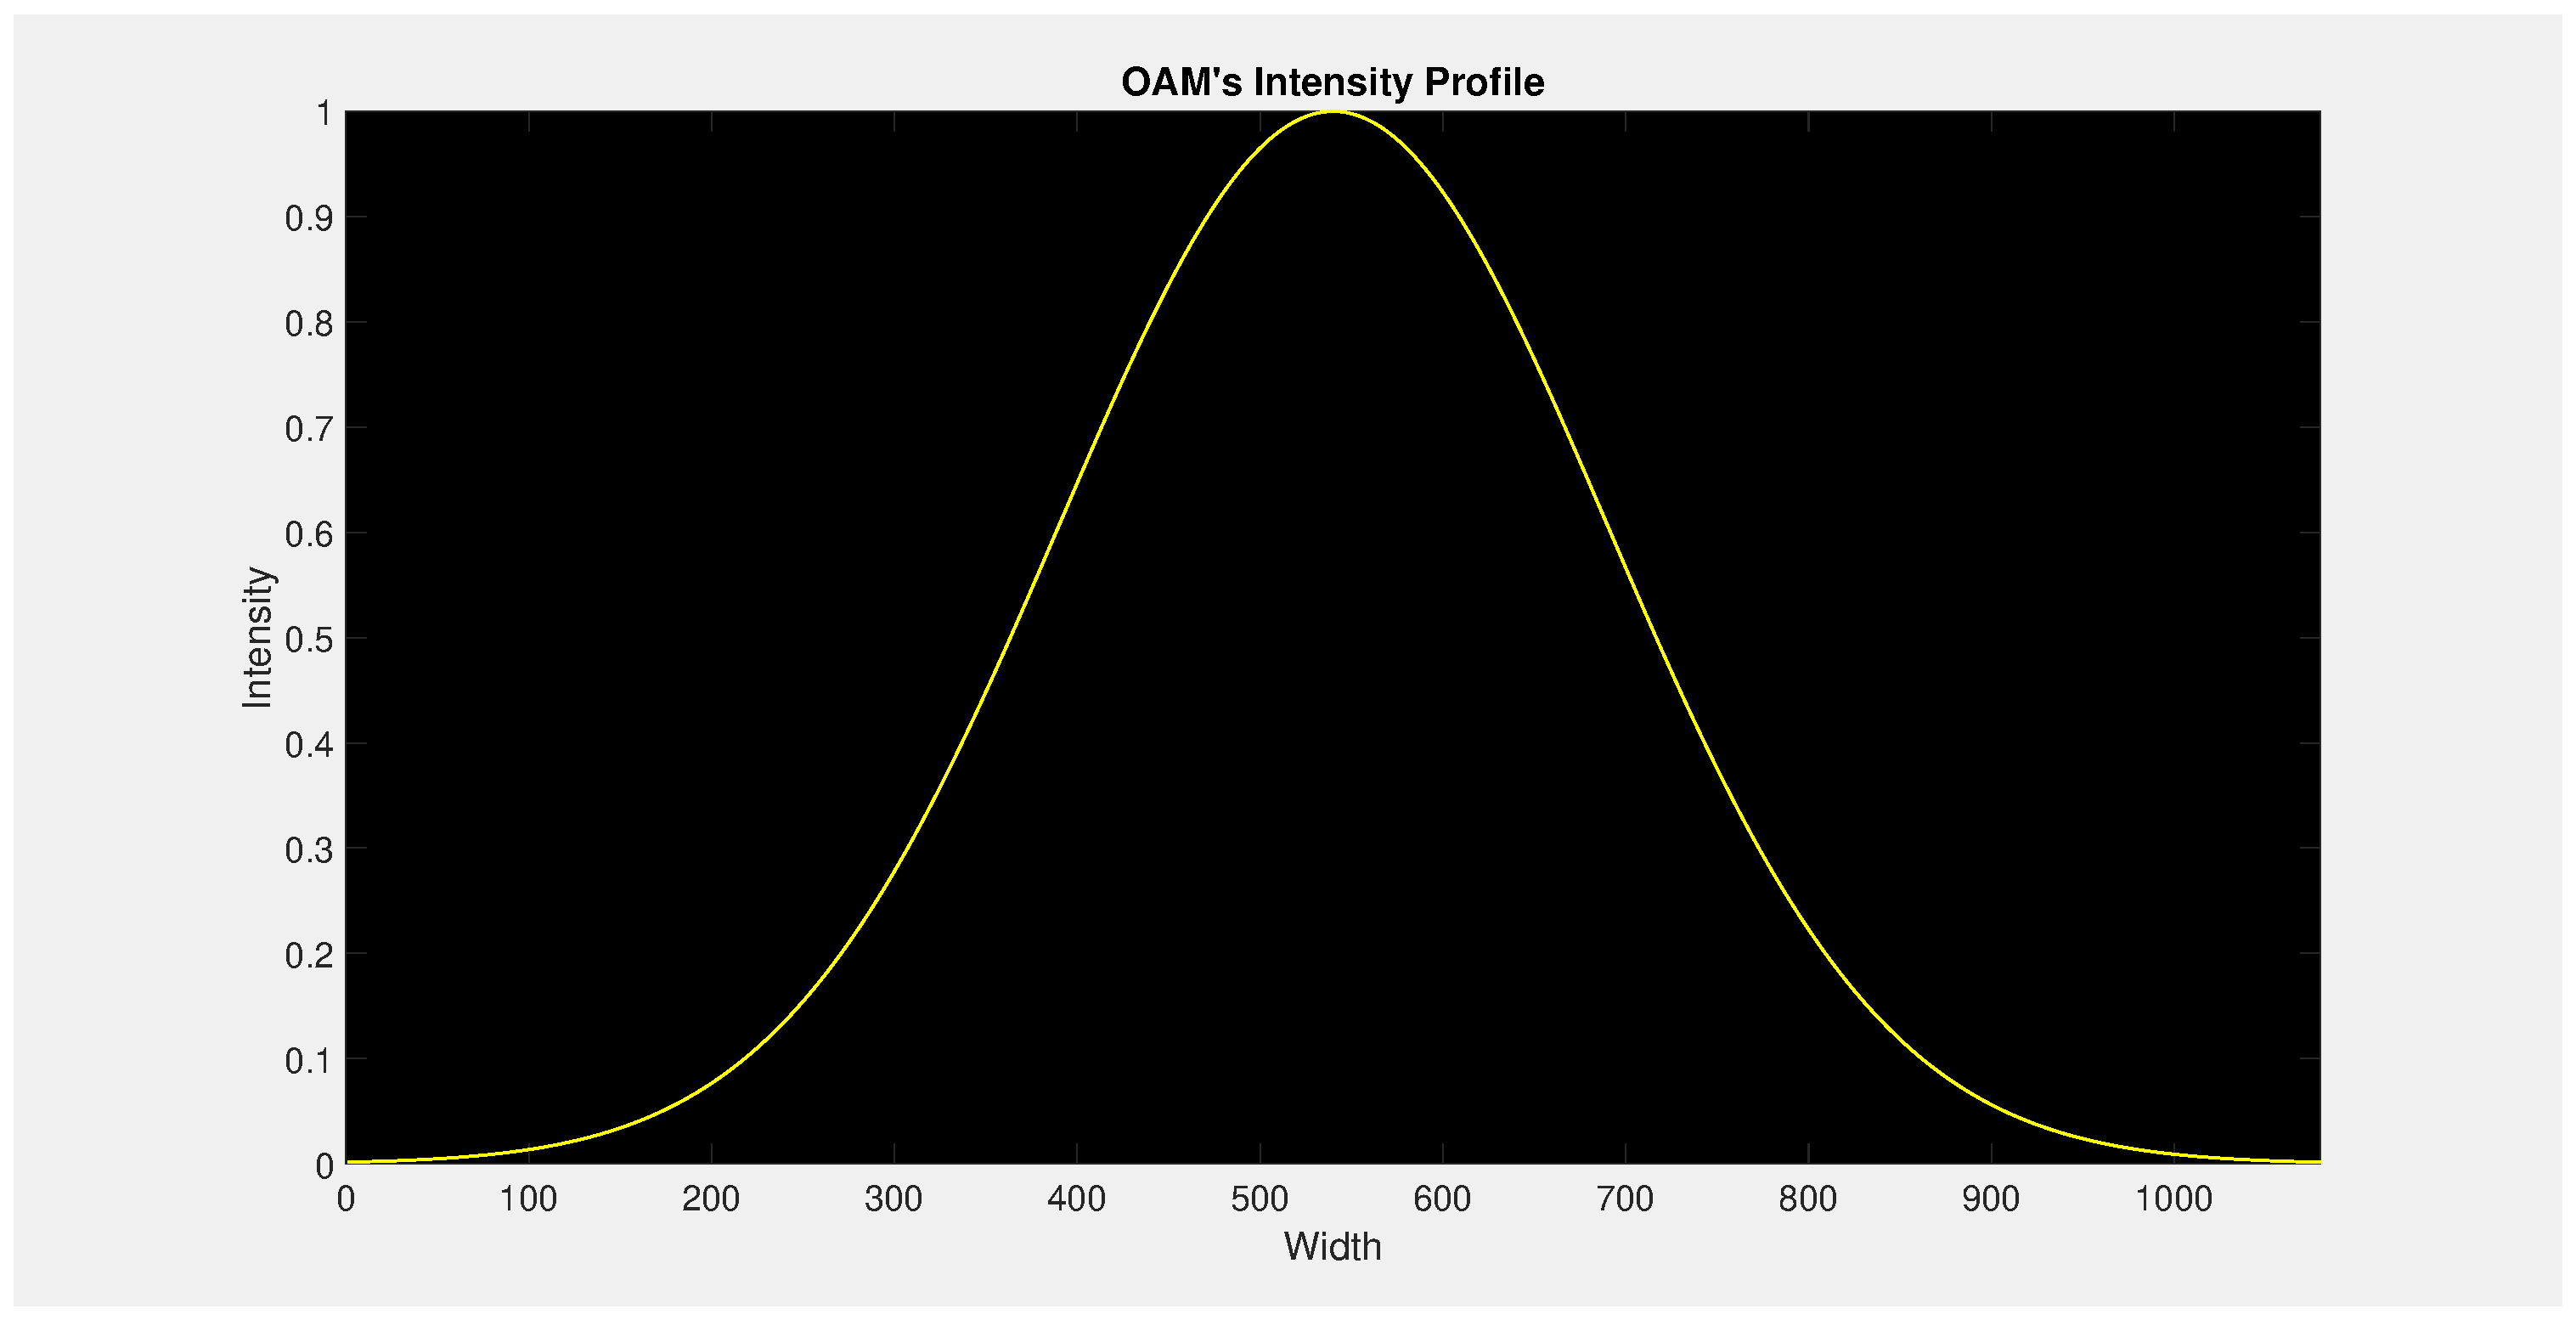
\includegraphics[width=\textwidth]{images/c02/OAM/Gauss_Profile.eps}
        \caption{Regular Gaussian beam's intensity profile.}
        \label{fig:example_Gaussian_profile}
    \end{subfigure}
    \hfill
    \begin{subfigure}[b]{0.45\textwidth}
        \centering
        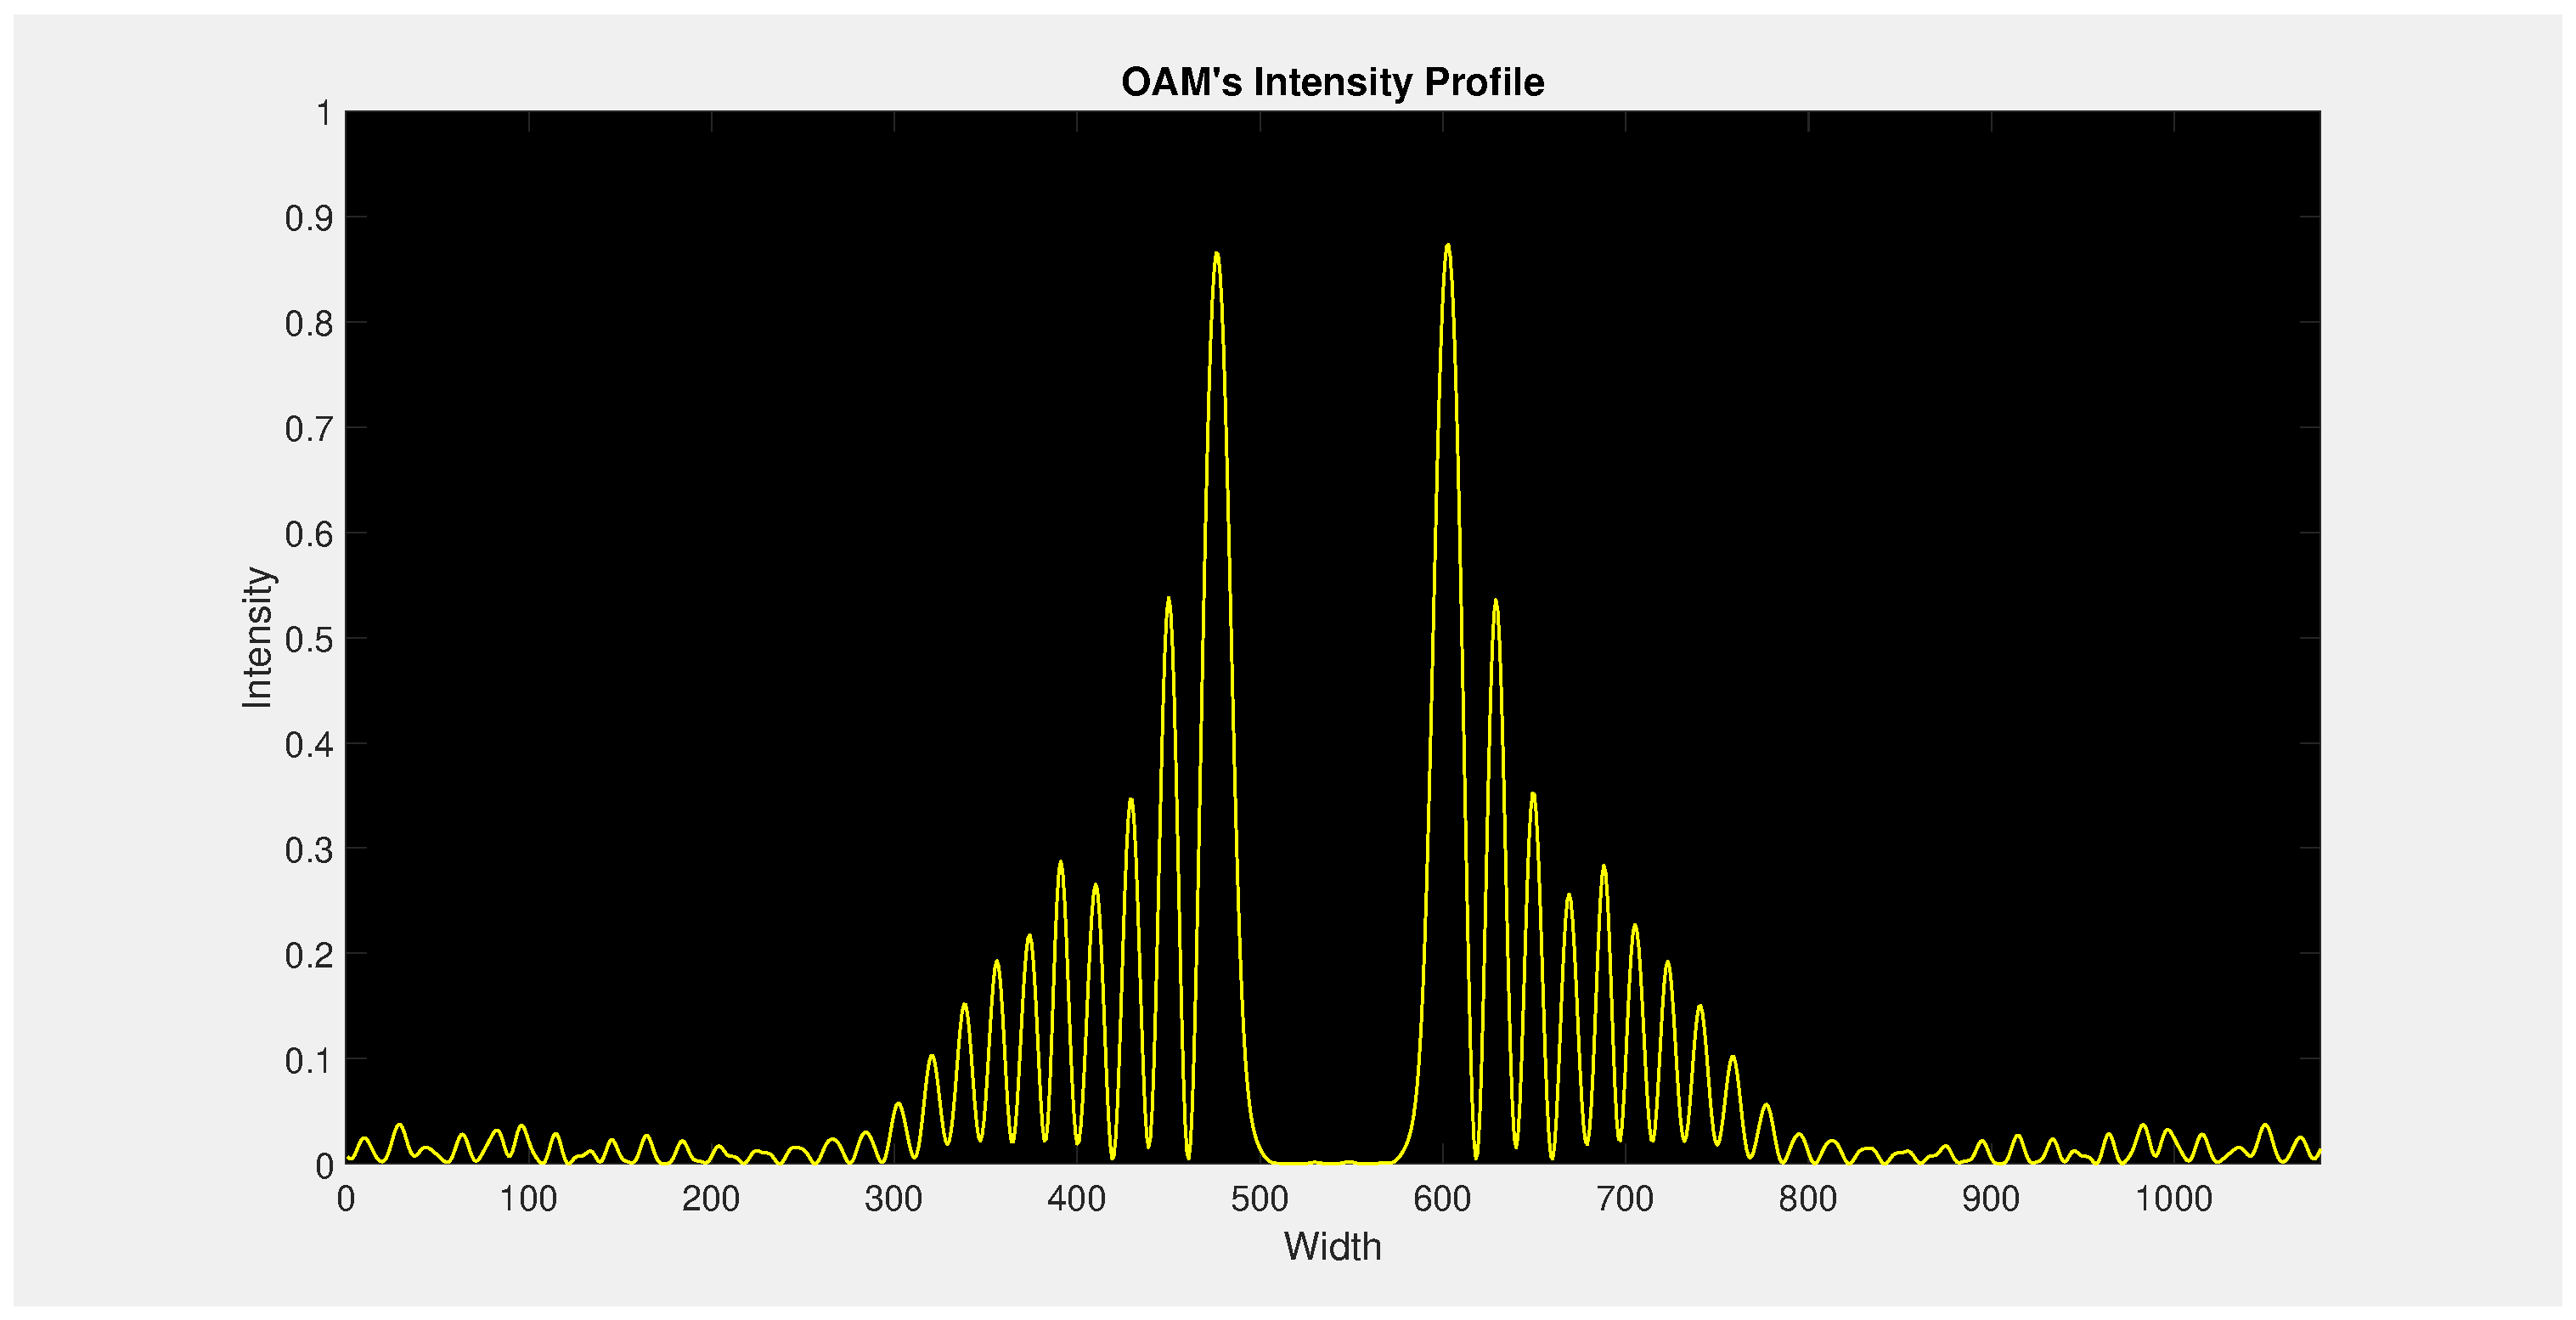
\includegraphics[width=\textwidth]{images/c02/OAM/Gaussian_Profile.eps}
        \caption{Intensity profile of the perfect vortex shown in figure (\ref{fig:Example_OAM}).}
        \label{fig:example_perfect_OAM_profile}
    \end{subfigure}
    \caption{Normalized intensity profiles. Notice how figure (\ref{fig:example_perfect_OAM_profile}) still follows the general shape of a Gaussian curve, as well as for each individual ring.}
    \label{fig:Example_Intesity_Profiles}
\end{figure}

\subsection{Making an OAM beam}
\label{c2:Making an OAM beam}

There are three commonly used methods to induce orbital angular momentum on a light beam. The first one is by combining Hermite-Gauss (HG) modes to generate Laguerre-Gaussian (LG) ones using a laser. Another one, is by using a spiral phase plate whose optical thickness varies linearly with the azimuthal angle. The final method consists of using a spatial light modulator (SLM)\footnote{An SLM is a device that allows one to modulate a beam of light through a projection, which can be controlled by a computer. It uses the same working principle of a transparency projection.} to project a \textit{phase mask}\footnote{Also referred to as \textit{hologram} or \textit{interference pattern plate}.} that sits in front of a typical laser beam and induces OAM on it. The phase mask is generated by the Laguerre-Gauss equation (\ref{Laguerre-Gauss Equation}) \cite{Anguita:08}.

\begin{figure}[htbp]
    \centering
    \begin{subfigure}[b]{0.3\textwidth}
        \centering
        \fbox{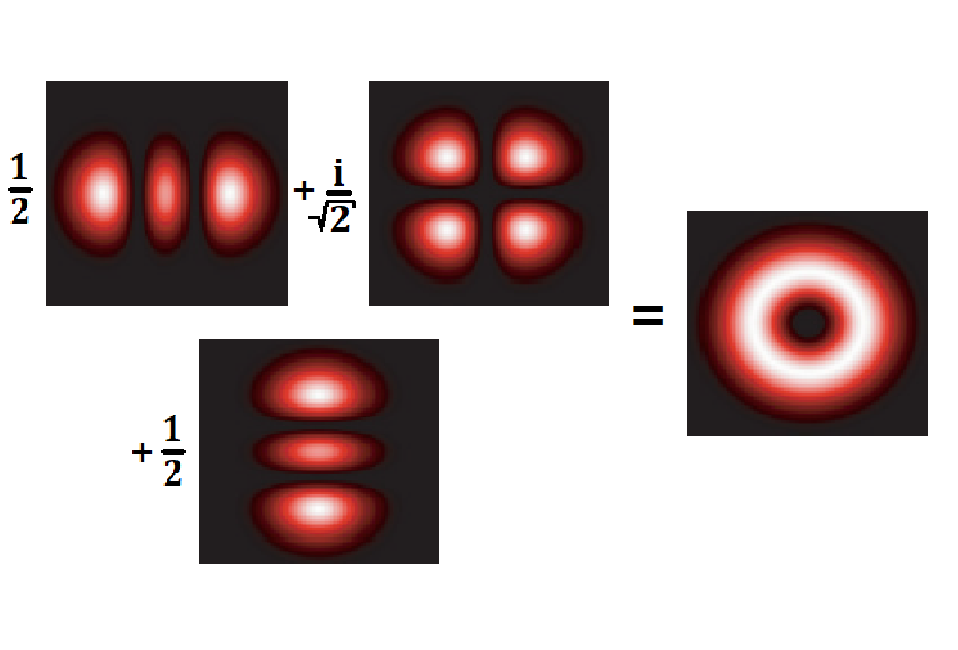
\includegraphics[width=\textwidth]{images/c02/OAM/HG_to_LG_resized.png}}
        \caption{First method: conversion from HG to LG modes \cite{Yao-Padgett:2011}.}
    \end{subfigure}
    \hfill
    \begin{subfigure}[b]{0.3\textwidth}
        \centering
        \fbox{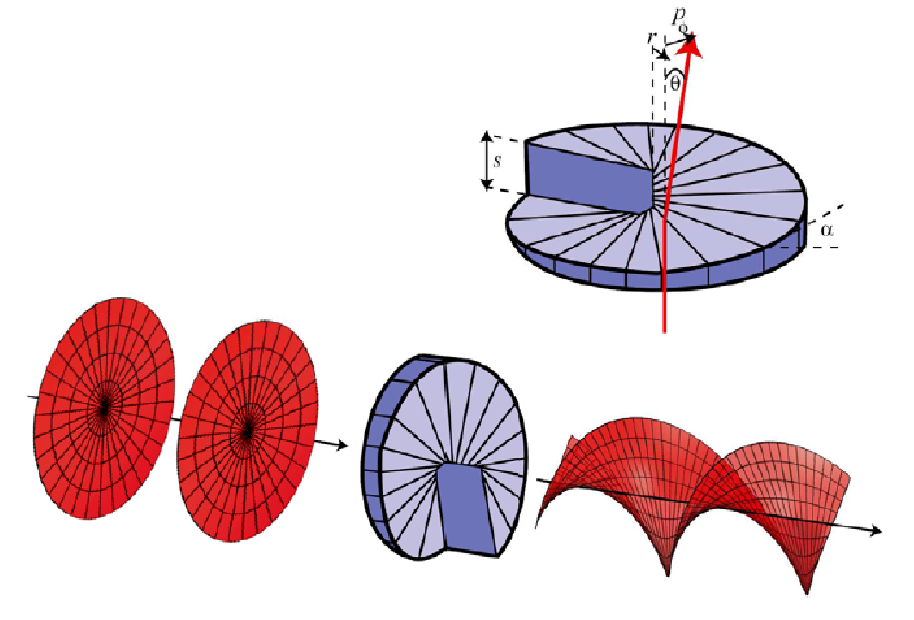
\includegraphics[width=\textwidth]{images/c02/OAM/OAM_Plate.PNG}}
        \caption{Second method: Using a spiral phase plate \cite{Yao-Padgett:2011}.}
    \end{subfigure}
    \hfill
    \begin{subfigure}[b]{0.3\textwidth}
        \centering
        \fbox{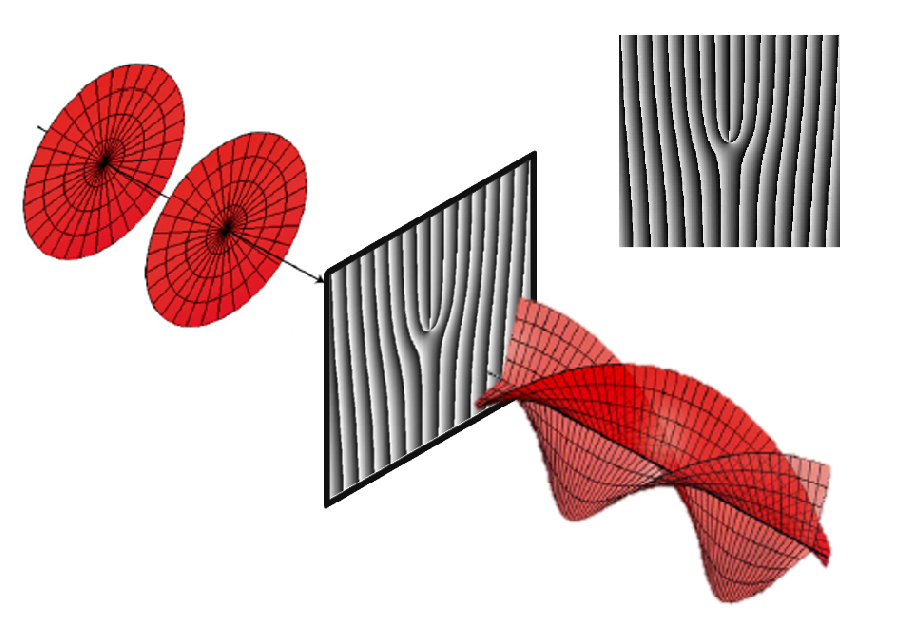
\includegraphics[width=\textwidth]{images/c02/OAM/Gaussian-Fork-OAM.png}}
        \caption{Third Method: Using a phase mask (Created by the author).}
    \end{subfigure}
    \caption{Illustration of all three methods to generate an optical vortex. Assuming each one is producing the same OAM's state, their outcomes should be the same vortex, in theory.}
    \label{fig:OAM_Generation_Methods}
\end{figure}

In the FICA\footnote{Spanish acronym for ``Facultad de Ingeniería y Ciencias Aplicadas''.} optics laboratory, the third method is preferred due to its simplicity and relatively cheap implementation, as the SLM's projection can change, allowing for flexibility in the variations of the experiments. Finally, because the SLM is controlled by a computer through a common DVI or HDMI cable, changing the setup is almost instantaneous without requiring physical modifications to the experiment table. Ultimately, to adhere as closely as possible to this condition, the work presented in this paper simulates this approach.

The Laguerre-Gauss equation that can generate different phase masks is \cite{Yao-Padgett:2011}:

\begin{eqnarray}
    LG_{\ell, p} = \sqrt{\frac{2p!}{\pi (p + |\ell|)!}}\frac{1}{w(z)}\left[ \frac{r\sqrt{2}}{w(z)} \right]^{|\ell|}exp\left[ \frac{-r^2}{w^2(z)} \right] L_p^{|\ell|} \left( \frac{2r^2}{w^2(z)} \right) exp[i\ell\phi]\nonumber\\exp\left[ \frac{ik_0r^2z}{2(z^2+z^2_R)} \right] exp \left[ -i(2p+|\ell|+1)\tan^{-1}{\left( \frac{z}{z_R} \right)} \right]
    \label{Laguerre-Gauss Equation}
\end{eqnarray}

Where the Gaussian's radius is given by the expression $w(z) = w(0)[(z^2+z^2_R)/z^2_R]^{1/2}$, $z$ is the beam's propagation distance, $w(0)$ is the beam's radius for $z=0$ (or beam ``waist''; see figure (\ref{fig:Gaussian_Beam_Waist})), $z_R$ is Rayleigh's range and $(2p+|\ell|+1)\tan^{-1}{(z/z_R)})$ is the Gouy phase\footnote{Defined as the phase changes that the beam experiments near its focal distance.}. The term $L_p^{|\ell|}(x)$ is a polynomial obtained from the Laguerre polynomials, described by the following expression:

\begin{equation}
    L_p^{|\ell|}(x) = (-1)^{|\ell|}\frac{d^{|\ell|}}{dx^{|\ell|}}L_{p+|\ell|}(x)
\end{equation}

Notice that Rayleigh's range $z_R$ is given by equation:

\begin{equation}
    z_R = \frac{\pi w_0^2n}{\lambda}
\end{equation}

Where $\lambda$ is the wavelength and $n$ is the medium's refractive index.

\begin{figure}[htbp]
    \centering
    \fbox{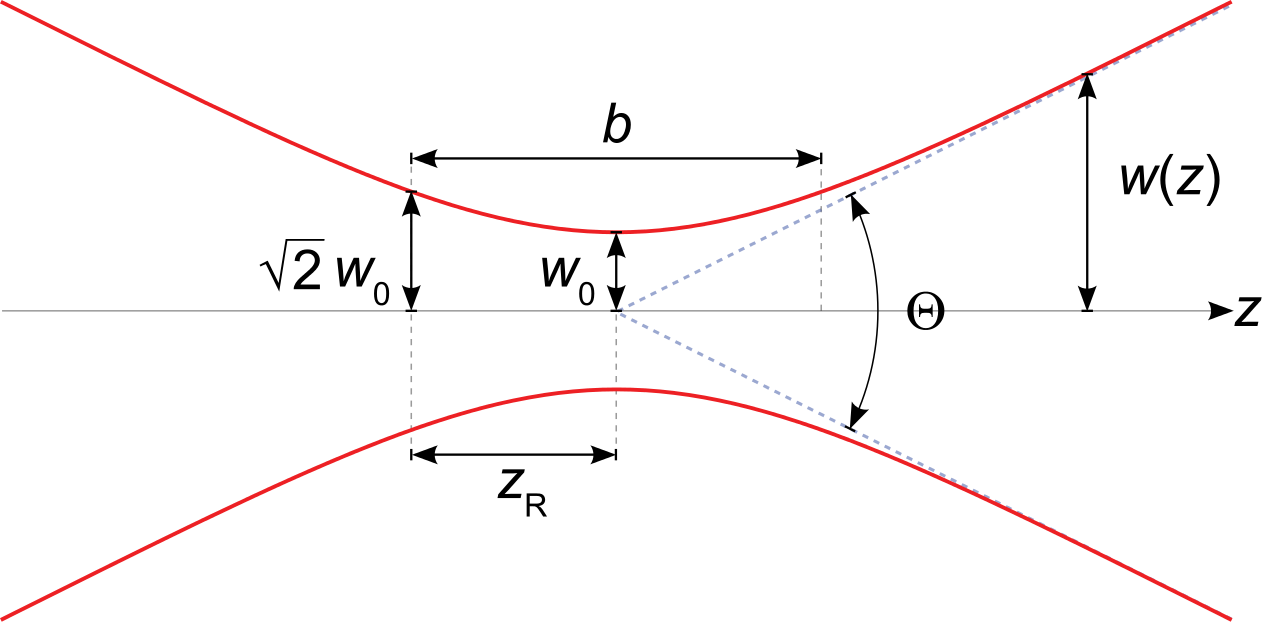
\includegraphics[width=8.5cm]{images/c02/OAM/GaussianBeamWaist.png}}
    \caption{Illustration of the Gaussian beam's waist \protect\cite{GaussianBeamParameters}.}
    \label{fig:Gaussian_Beam_Waist}
\end{figure}

As it can be seen, the two input arguments of equation (\ref{Laguerre-Gauss Equation}) are $\ell$ and $p$, the latter representing the number of rings of the vortex. Examples of vortices with different values for these parameters are shown in figure (\ref{fig:OAMs_given_L_and_P}).

\begin{figure}[htbp]
    \centering
    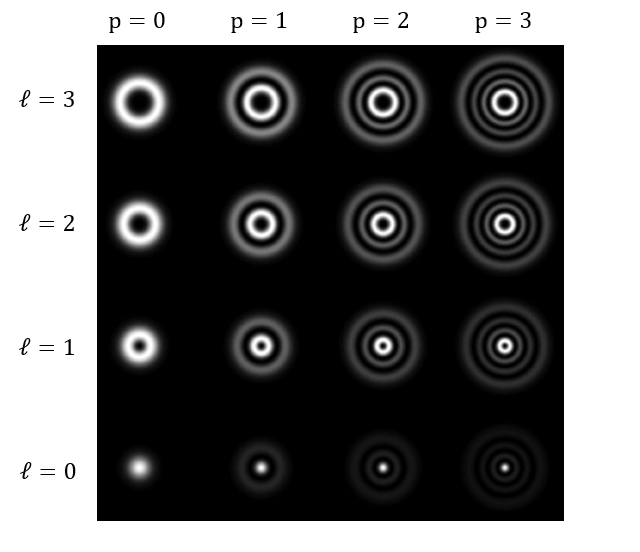
\includegraphics[width=9cm]{images/c02/OAM/OAM_given_L_and_P.png}
    \caption{Resulting optical vortices for different $\ell$ and $p$ values for equation (\ref{Laguerre-Gauss Equation}) \protect\cite{OAM_states_Carbone:2013}.}
    \label{fig:OAMs_given_L_and_P}
\end{figure}

\newpage
The phase masks created by this equation correspond to the complex field of equation (\ref{Light Equation}) (See figure (\ref{fig:lighteq_to_images})). As the light equation of these beams is propagated, its intensity and complex fields are altered (for more detail on how exactly they are altered, refer to section (\ref{c2:Near and Far Field Propagation}). The intensity field of the same light equation is what we are able to see with our own eyes directly; in this case, this is the OAM beam, like the ones shown in figure (\ref{fig:Example_OAM}).

\begin{figure}[htbp]
    \centering
    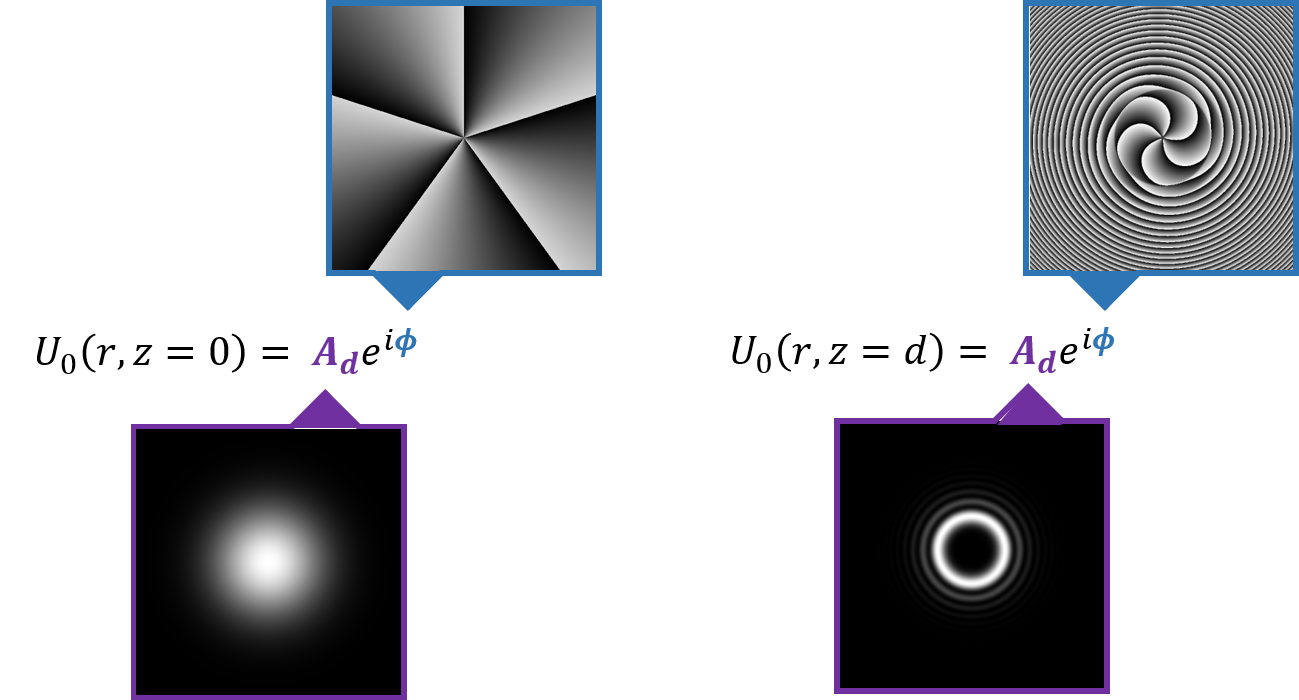
\includegraphics[width=11cm]{images/c02/OAM/Light_Equation_Images.png}
    \caption{Relationship between the terms of the light equation (fields) and their respective images. The phase mask corresponds to the complex field and the OAM corresponds to the intensity field.}
    \label{fig:lighteq_to_images}
\end{figure}

\newpage
Hence, what essentially plays out is that one projects a phase mask through an SLM controlled by a computer onto a Gaussian laser beam, with the resulting beam being an OAM beam.

\begin{figure}[htbp]
    \centering
    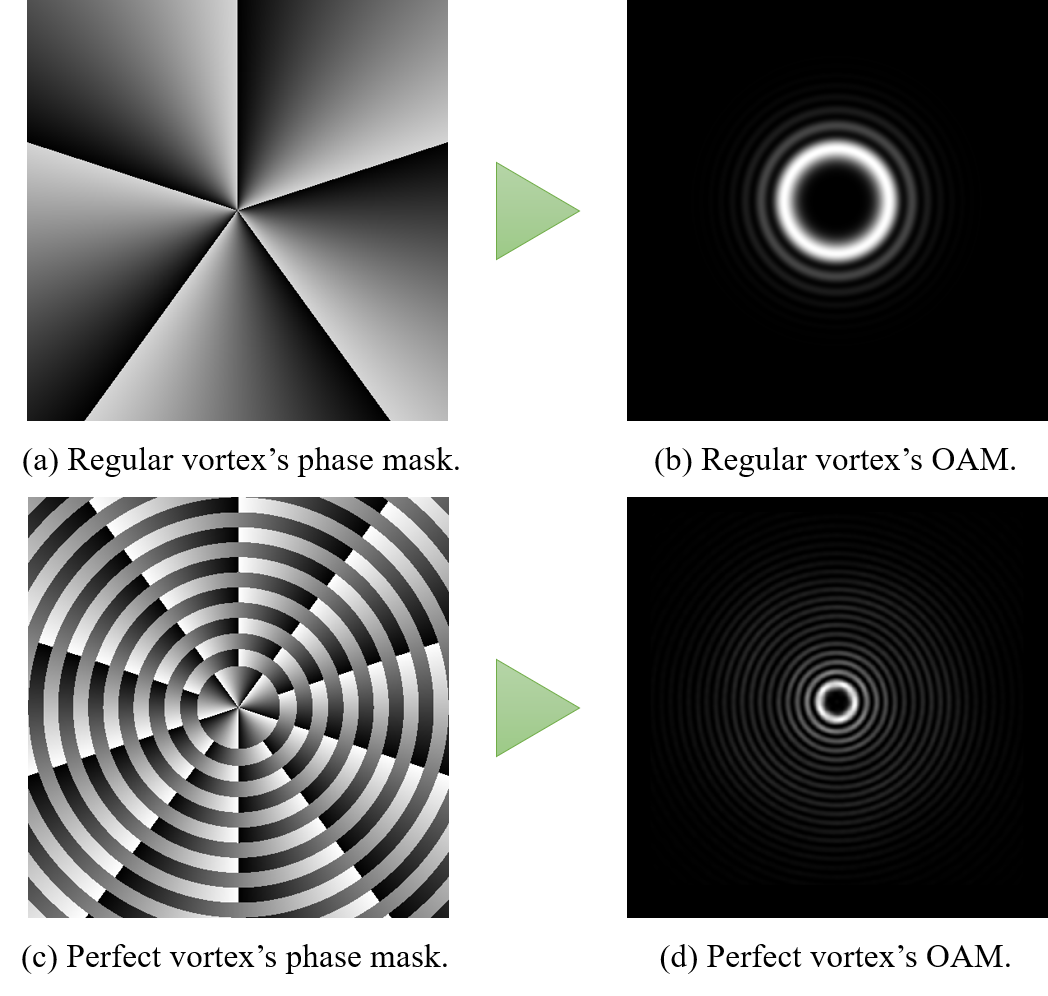
\includegraphics[width=10cm]{images/c02/OAM/PhaseMasks_to_OAM.png}
    \caption{Relationship between the phase masks projected by the SLM and the resulting OAMs, or intensity fields.}
    \label{fig:PM2OAM}
\end{figure}

For the particular case of perfect OAMs, their phase mask is created through the Optimal Phase Element method. It seeks to concentrate most of the beam's intensity onto the main ring, given by equation ().

\begin{equation}
    U(r,\varphi) = sgn(J_\ell(\alpha r))e^{il\Phi(r,\varphi)}
\end{equation}

Where $r = \sqrt{x^2 + y^2}$ and $\Phi(r,\varphi) = circ \left( \frac{r}{R} \right) il\varphi$; $R$ is the circular aperture's radius and $J_\ell$ is the first order Bessel function of order $\ell$. Finally, $circ \left( \frac{r}{R} \right)$ is 1 when r is less than or equal to the aperture R, and is 0 if its greater.


\newpage
\section{Near-Field and Far-Field Propagation Models}
\label{c2:Near and Far Field Propagation}

In order to simulate the propagation of an OAM beam, it is necessary to define the near-field and far-field diffraction models mathematically. They are used to resemble, as accurately as possible, the diffraction pattern generated by light passing through an aperture, assuming that the light source is coherent, which means that it emanates monochromatic wavefronts like that from a laser. 

The reason to distinguish between both near and far field scenarios, come from observing the changes that the outcome's intensity pattern experiences as the surface onto the which is projected is placed further away from the slit. A visual representation of this phenomenon is shown in figure (\ref{fig:Diffraction-Distinction}).

\begin{figure}[htbp]
    \centering
    \fbox{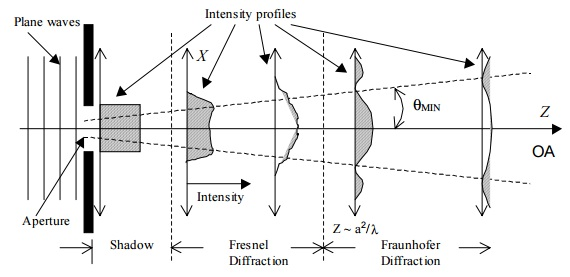
\includegraphics[width=10cm]{images/c02/Propagation/Fresnel-Fraunhoffer_Diffraction.jpg}}
    \caption{Illustration of varying intensity profiles as the projection is placed further from the slit \protect\cite{Near-Far_Field_Diff}.}
    \label{fig:Diffraction-Distinction}
\end{figure}

There is a critical distance that serves to determine whether near field diffraction or far field one are to be used in a certain scenario. This distance is given by equation (\ref{near-far-field}) and it relates the beam's size and wavelength.

\begin{equation}
    d = \frac{2D^2}{\lambda}
    \label{near-far-field}
\end{equation}

Here, $d$ is the critical distance and $D$ is the beam's radius. Although there is not a more accurate definition, it is accepted that near field and far field are given by their relation with the critical distance, as follows.

\begin{eqnarray}
    z &>& d \implies \textrm{near field}\\
    z &>>& d \implies \textrm{far field}
\end{eqnarray}

In this fashion, the Fresnel diffraction or integral is defined as the contribution of each point $U_s$ from the plane at the beginning of the propagation, which is for $z = 0$ and defined by axes $x'$ and $y'$, onto the point $U_0$ within the propagated plane defined by axes $(x,y)$, as shown in figure (\ref{fig:Propagation_Diagram}).

\begin{figure}[htbp]
    \centering
    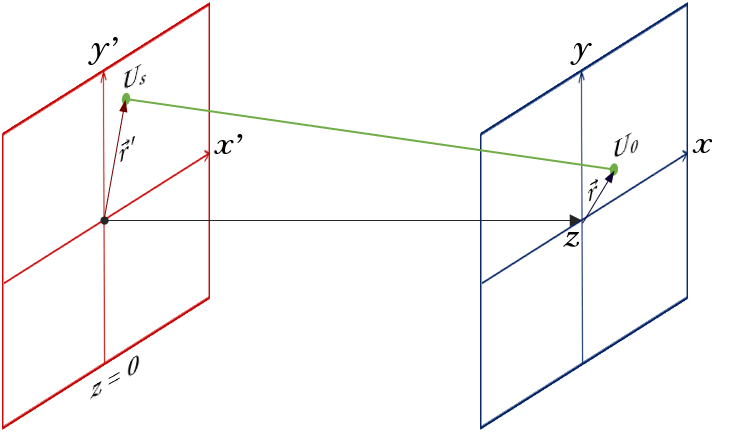
\includegraphics[width=9cm]{images/c02/Propagation/Propagation.png}
    \caption{Diagram of the propagation of a coherent wavefront from one plane onto another (Created by the author).}
    \label{fig:Propagation_Diagram}
\end{figure}

\begin{equation}
    U_0(x,y) = \frac{1}{i\lambda}\int_{-\infty}^{\infty}\int_{-\infty}^{\infty}\frac{U_s(x',y')e^{ik|\overrightarrow{r}-\overrightarrow{r}'|}}{|\overrightarrow{r}-\overrightarrow{r}'|}dx'dy'
    \label{Fresnel Integral}
\end{equation}

Here, the expression $|\overrightarrow{r}-\overrightarrow{r}'| = \sqrt{(x-x')^2+(y-y')^2+z^2}$ and $k = \frac{2\pi}{\lambda}$. We can simplify equation (\ref{Fresnel Integral}) by using the binomial expansion and paraxial approximation, respectively.

\begin{equation}
    \sqrt{(x-x')^2+(y-y')^2+z^2} = z\sqrt{1 + \left( \frac{x - x'}{z} \right)^2 + \left( \frac{y - y'}{z} \right)^2}
    \label{Binomial Expansion}
\end{equation}

\begin{equation}
    z\sqrt{1 + \left( \frac{x - x'}{z}^2 \right) + \left( \frac{y - y'}{z}^2 \right)} \approx z \left( 1 + \frac{1}{2} \left( \frac{x - x'}{z} \right)^2 + \frac{1}{2} \left( \frac{y - y'}{z} \right)^2 \right)
    \label{Paraxial Approximation}
\end{equation}

Considering that the propagation distance is significantly greater than the ``displacement'' that $U_0$ endures, with respect to $U_s$ it can be assumed that $z >> (x-x')$ and $z >> (y-y')$. This allows to nullify the terms in equation (\ref{Paraxial Approximation}) being divided by z, leaving the equation as $\approx z(1+0+0) = z$. Notwithstanding, is this approach in the denominator of equation (\ref{Fresnel Integral}), as it is scaled by $k$, which can enlarge errors not considered by the approximation and negatively alter the outcome. Taking this into consideration, the near field approximation is left obtained.

\begin{equation}
    U_0(x,y) = \frac{1}{i\lambda z}\int_{-\infty}^{\infty}\int_{-\infty}^{\infty}U_s(x',y')e^{ikz \left( 1 + \frac{1}{2} \left( \frac{x - x'}{z} \right)^2 + \frac{1}{2} \left( \frac{y - y'}{z} \right)^2 \right)}dx'dy'
\end{equation}

Finally, by moving the $x'$-and-$y'$-independent terms out of the integral, we are left with the simplified near field approximation.

\begin{equation}
    U_0(x,y) = \frac{e^{ikz}}{i\lambda z}e^{\frac{i\pi}{\lambda z}(x^2+y^2)}\int_{-\infty}^{\infty}\int_{-\infty}^{\infty}U_s(x',y')e^{\frac{i\pi}{\lambda z}(x'^2+y'^2)}e^{-i\frac{2\pi}{\lambda z} (xx'+yy')}dx'dy'
    \label{Near Field Approximation}
\end{equation}

On the other hand, the far field approximation assumes instead that the propagation distance is significantly greater than the the projection $U_0$ itself, or mathematically, $z >> x'^2$ and $z > y'^2$. Hence, the term $e^{\frac{i\pi}{\lambda z}(x'^2+y'^2)} \rightarrow 1$ because:

\begin{equation}
    \frac{x'^2}{z} \rightarrow 0, \frac{y'^2}{z} \rightarrow 0
\end{equation}

Therefrom, Fraunhoffer's approximation is obtained.

\begin{equation}
    U_0(x,y) = \frac{e^{ikz}}{i\lambda z}e^{\frac{i\pi}{\lambda z}(x^2+y^2)}\int_{-\infty}^{\infty}\int_{-\infty}^{\infty}U_s(x',y')e^{-i\frac{2\pi}{\lambda z} (xx'+yy')}dx'dy'
    \label{Far Field Approximation}
\end{equation}

\newpage
It is also possible to rewrite this equation by using the Fourier transform, which is specially useful for MATLAB. Notice how the double integral resembles the 2D Fourier transform definition. By defining the variables $u = \frac{x}{\lambda z}$ and $v = \frac{y}{\lambda z}$, then this double integral can designate the Fourier Transform of some function $f_s(x',y')$.

\begin{equation}
    U_0(x,y) = \frac{e^{i\frac{2\pi}{\lambda}}z}{i\lambda z}e^{i\pi \lambda z(x^2+y^2)}F_s(\frac{x}{\lambda z},\frac{y}{\lambda z})
\end{equation}
